\documentclass[11pt]{article}
\usepackage[a4paper, portrait, margin=1in]{geometry}

\newcommand{\myname}{Tom Sydney Kerckhove}
\newcommand{\mynetzh}{tomk}
\newcommand{\myleginr}{15-908-064}

\newcommand{\javafile}[1]{\footnote{\url{https://gitlab.inf.ethz.ch/\mynetzh/asl-fall16-project/blob/master/asl/src/ch/ethz/asl/#1.java}}}
\newcommand{\plot}[1]{plots/#1}
\newcommand{\asset}[1]{assets/#1}


\newcommand{\java}[1]{\mintinline{java}{#1}}


\usepackage{float}
\usepackage{hyperref}
\usepackage{tikz}
\usetikzlibrary{shapes}
\usetikzlibrary{patterns}



% Report Checklist:


% Define service, waiting time and map them onto design for each model.
% Explain where each number comes from.








\begin{document}

\title{Advanced Systems Lab (Fall'16) -- Third Milestone}

\author{Name: \emph{\myname}\\Legi number: \emph{\myleginr}}

\date{
\vspace{4cm}
\textbf{Grading} \\
\begin{tabular}{|c|c|}
\hline  \textbf{Section} & \textbf{Points} \\ 
\hline  1 &  \\ 
\hline  2 &  \\ 
\hline  3 &  \\ 
\hline  4 &  \\ 
\hline  5 &  \\ 
\hline \hline Total & \\
\hline 
\end{tabular} 
}

\maketitle
\newpage

\section{Overview}

This report is the third installment in a series of three reports for the Advanced System Lab course.
The two previous reports considered the building of a middleware and experimentation.
This report will focus on modelling the middleware.

A model of the situation can be found in figure \ref{ref:complete-system}.

\begin{figure}[H]
  \centering
	
  \begin{tikzpicture}
    \node[anchor=south west,inner sep=0] (image) at (0,0) {\includegraphics[width=0.5\textwidth]{\asset{architecture.png}}};
    \begin{scope}[x={(image.south east)},y={(image.north west)}]
			\draw (-0.7,0.5) circle (1cm) node (C) {Clients};
			\node (N) at (-0.3,0.5) [cloud, draw,cloud puffs=10,cloud puff arc=120, aspect=2, inner ysep=1em] {network};
			\draw [->, thick] (C) -- (N) -- (image);
    \end{scope}
  \end{tikzpicture}
  \caption{Complete view of the system}
  \label{ref:complete-system}
\end{figure}

\section{System as One Unit}\label{sec:system-one-unit}

% Length: 1-2 pages

% Build an M/M/1 model of your entire system based on the stability trace that you had to run for the first milestone.
% Explain the characteristics and behavior of the model built, and compare it with the experimental data (collected both outside and inside the middleware).
% Analyze the modeled and real-life behavior of the system (explain the similarities, the differences, and map them to aspects of the design or the experiments).
% Make sure to follow the model-related guidelines described in the Notes!

\subsection{Boundaries of M/M/1 model}

To make a M/M/1 model of the entire system, we have to treat the system under test as a black box.
The black box is drawn from the middleware, across the network on the network on the server side and across the servers.

This black box seemed the most appropriate.
Adding the network on the client-side to the black box would add more network-traveling to the service that we are modelling.
On the other hand, drawing the black box around the middleware only makes it hard to define what the service of the model is.

In figure \ref{fig:mm1-black-box}, there is an illustration of the black box used for this model.

\begin{figure}[H]
  \centering
  \begin{tikzpicture}
    \node[anchor=south west,inner sep=0, opacity=0.4] (image) at (0,0) {\includegraphics[width=0.5\textwidth]{\asset{architecture.png}}};
    \begin{scope}[x={(image.south east)},y={(image.north west)}]
			\draw (-0.7,0.5) circle (1cm) node (C) {Clients};
			\node (N) at (-0.3,0.5) [cloud, draw,cloud puffs=10,cloud puff arc=120, aspect=2, inner ysep=1em] {network};
			\draw [->, thick] (C) -- (N) -- (image);
			\draw [pattern=north west lines, pattern color=blue, fill=black, fill opacity=0.3, text opacity=1] (0,0) rectangle (1.05,1.05);
    	\node[anchor=south west,inner sep=0] (image) at (0,0.31) {\includegraphics[width=0.5\textwidth]{\asset{mm1.png}}};
    \end{scope}
  \end{tikzpicture}
  \caption{Black box system for M/M/1 model}
  \label{fig:mm1-black-box}
\end{figure}


\subsection{Parameter estimation}

Next we pretend that everything in this black box corresponds to a system as modeled by an M/M/1 model, and try to estimate the parameters $\lambda$ and $\mu$ of the M/M/1 model.
To justify the following estimation of the parameters, we rely on the fact that we are dealing with a closed system.

The model parameters will be estimated on a stability trace experiment that was run in the first part of the project.
However, due to updates to the system, this experiment has had to be re-run.
The details of the configuration can be found in figure \ref{fig:sut-stability-trace}.

\begin{figure}[H]
  \centering
  \input{\genfile{remote-stability-trace-table.tex}}
  \caption{Stability trace}
  \label{fig:sut-stability-trace}
\end{figure}

\subsubsection{Estimation of the arrival rate $\lambda$}

The arrival rate $\lambda$ is estimated by the average\footnote{over the seconds of the trace} throughput as seen by the clients.
Indeed, because we are dealing with a closed system, the rate at which requests arrive at the black box is exactly equal to the rate at which requests get processed.

\subsubsection{Estimation of the service rate $\mu$}

The service rate $\mu$ is estimated by the maximum throughput throughput as seen by the clients over all the 1 second intervals of the experiment.
This can be justified by realising that the service rate is the maximum speed at which the system can process requests.
This means that taking the maximum throughput will yield a lower bound for the service rate.
Because we consider many one second intervals, this estimation should give us a relatively accurate lower-bound for the service rate.

\subsection{Comparison with experimental results}

In figure \ref{fig:mm1-model}, we can see the M/M/1 model that was built according to guidelines of the previous subsection.
On the left-hand side we can see the input parameters and output measures as predicted by the model.
On the right-hand side we can see a comparison with data gathered from the system.

\begin{figure}[H]
  \centering
  \input{\model{remote-stability-trace-mm1.tex}}
  \caption{M/M/1 model}
  \label{fig:mm1-model}
\end{figure}

It is important to note that 'response time' means the total time before the black box replies.
It has little to do with what the clients call the 'response time'.
The mean waiting time on the left means the time that a request spends in the M/M/1 model queue before being processed.

The data that these predictions are compared with are the best available data for the comparison:
The mean response time is compared to the difference between the average total time spent between receiving a request and sending a response by the middleware.
The mean waiting time is compared to the time between being enqueued and being dequeued by a request.

\subsection{Mapping between comparison and system components}

The M/M/1 model is a very limited model that cannot accurately represent the black box that it is covering.
However, it can still provide some insight in the system at hand.

In the second part of figure \ref{fig:mm1-model}, we find some data gathered from experiments performed with the real system.
The 'response time' predicted by the model can be compared with the 'response time' (total time between receiving a request and responding to the request).
As we can see the real response time is much higher than the predicted response time.
This makes sense as the model does not take parallelisation into account.

Nevertheless, there are some interesting observations to be made.

TODO MENTION ACTUAL NUMBERS WHEN THE DATA IS FINAL.

The model predicts a number of jobs in the queue and in the system.
The corresponding data of the real system is as follows.
Given that we are dealing with a closed system, there are approximately as many jobs in the system as there are (virtual) clients.
Similarly, given this approximation, there are approximately as many jobs in the system's queue(s) as there are are in the system, minus the amount that are being handled at the moment.
The number of jobs that are currently being handled is approximately equal to the total number of workers in the system.

The predicted number of jobs on the queue and in the system is much smaller than these estimates, but interestingly the ratio between the number of jobs in on the queue and the number of jobs in the system are remarkably similar.
This makes sense because both the queues and the handling of queues are parallelised in the real system.

Second, since there are many \TODO{how many} threads dequeuing from the same queue, it should hold that the predicted queueing time  times that number equals the actual queuing time.
\TODO{WHY}
We that this is in fact the case \TODO{show numbers}!

\TODO{other connections}

\section{Analysis of System Based on Scalability Data}\label{sec:analysis-scalability}

% Length: 1-4 pages

% Starting from the different configurations that you used in the second milestone, build M/M/m queuing models of the system as a whole. Detail the characteristics of these series of models and compare them with experimental data. The goal is the analysis of the model and the real scalability of the system (explain the similarities, the differences, and map them to aspects of the design or the experiments). Make sure to follow the model-related guidelines described in the Notes!

\subsection{Boundaries of M/M/m models}

In figure \ref{fig:mmm-black-box}, there is an illustration of the black box used for this model.

\begin{figure}[H]
  \centering
  \begin{tikzpicture}
    \node[anchor=south west,inner sep=0, opacity=0.4] (image) at (0,0) {\includegraphics[width=0.5\textwidth]{\asset{architecture.png}}};
    \begin{scope}[x={(image.south east)},y={(image.north west)}]
			\draw (-0.7,0.5) circle (1cm) node (C) {Clients};
			\node (N) at (-0.3,0.5) [cloud, draw,cloud puffs=10,cloud puff arc=120, aspect=2, inner ysep=1em] {network};
			\draw [->, thick] (C) -- (N) -- (image);
			\draw [pattern=north west lines, pattern color=blue, fill=black, fill opacity=0.3, text opacity=1] (0,0) rectangle (1.05,1.05);
    	\node[anchor=south west,inner sep=0] (image) at (0,0.19) {\includegraphics[width=0.5\textwidth]{\asset{mmm.png}}};
    \end{scope}
  \end{tikzpicture}
  \caption{Black box system for M/M/m model}
  \label{fig:mmm-black-box}
\end{figure}

\begin{figure}[H]
  \centering
  \includegraphics[width=\textwidth]{\plot{remote-replication-effect-mmm-model.png}}
\end{figure}


\section{System as Network of Queues}\label{sec:network-of-queues}

% Length: 1-3 pages

% Based on the outcome of the different modeling efforts from the previous sections, build a comprehensive network of queues model for the whole system. Compare it with experimental data and use the methods discussed in the lecture and the book to provide an in-depth analysis of the behavior. This includes the identification and analysis of bottlenecks in your system. Make sure to follow the model-related guidelines described in the Notes!

One queue at the front of the middleware, for incoming requests.
This queue is hidden behind java's async io functionality, but it's still there.
One MM1 queue per server, because we set memcached's number of threads to 1 and they each have a queue for incoming requests.

Per server also the following queues:
- an M/M/1 for writes
- an M/M/T for reads, where T is the number of threads per read queue.

We don't model anything more low-level than these systems. No CPU queue, no network queue, etc.

\TODO{make a nice illustration of this.}

\begin{figure}[H]
  \centering
  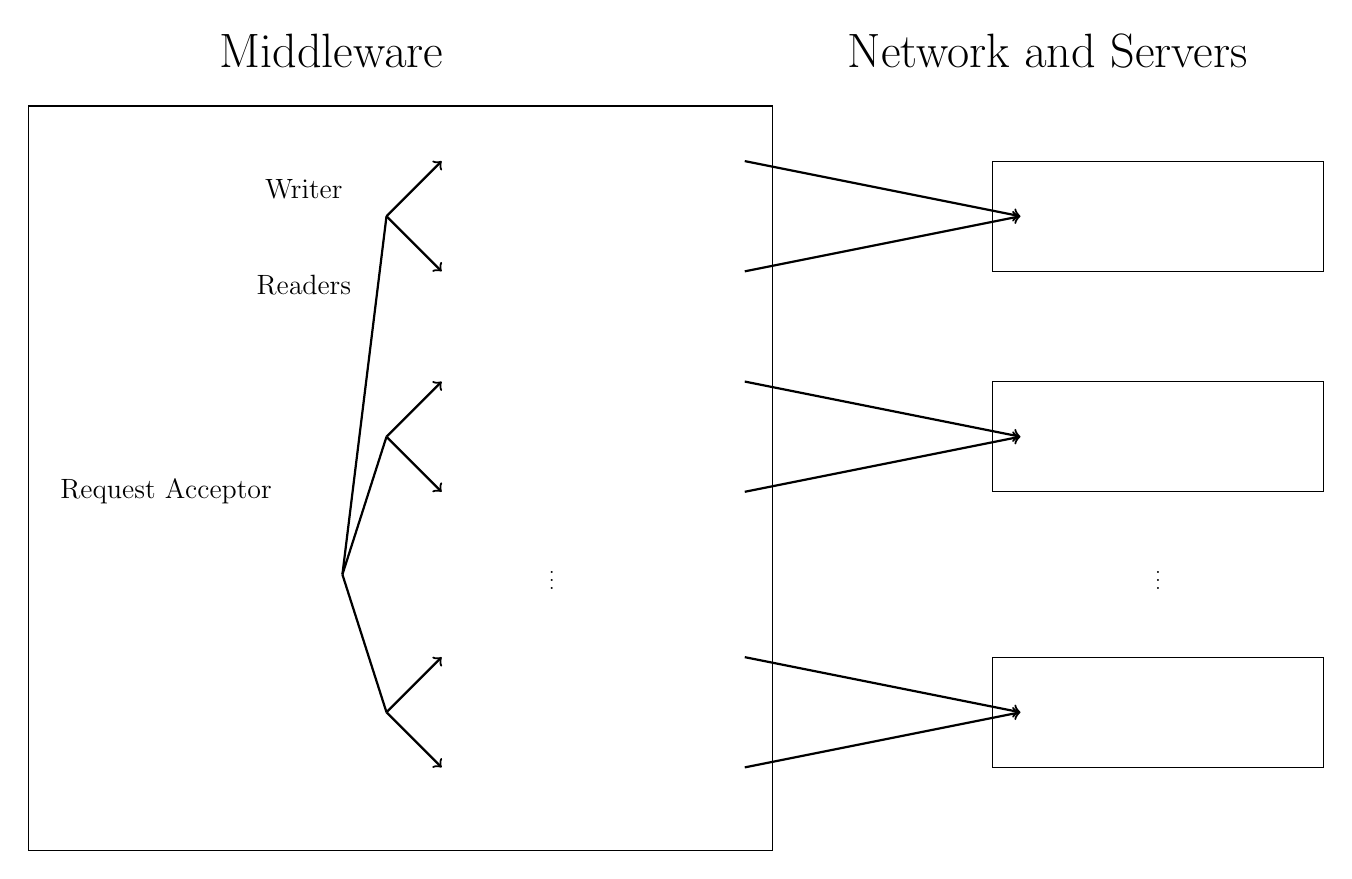
\begin{tikzpicture}[scale=0.7, every node/.style={scale=0.7}]
    % Connection accepter and initial reader
    \node at (9,2) {\Large Request Acceptor};
    \mmoqueue{200}{0}
    
    % Worker queues
    \node at (11.5,5.75) {\Large Readers};
    \node at (11.5,7.5) {\Large Writer};

		\draw [thick] (12.2,0.5) -- (13,7);
		\draw [->, thick] (13,7) -- (14,8);
		\draw [->, thick] (13,7) -- (14,6);
    \mmoqueue{400}{200}
    \mmmqueue{400}{150}
		\draw [thick] (12.2,0.5) -- (13,3);
		\draw [->, thick] (13,3) -- (14,4);
		\draw [->, thick] (13,3) -- (14,2);
    \mmoqueue{400}{100}
    \mmmqueue{400}{50}

    \node at (12,10) {\Huge Middleware};
    \node at (16,0.5) {\bm{$\vdots$}};

		\draw [thick] (12.2,0.5) -- (13,-2);
		\draw [->, thick] (13,-2) -- (14,-1);
		\draw [->, thick] (13,-2) -- (14,-3);
    \mmoqueue{400}{-50}
    \mmmqueue{400}{-100}

    \draw (6.5,-4.5) rectangle (20,9);

    % Server queues
		\draw [->, thick] (19.5,8) -- (24.5,7);
		\draw [->, thick] (19.5,6) -- (24.5,7);
    \mmoqueue{700}{185}
    \draw (24,6) rectangle (30,8);

		\draw [->, thick] (19.5,2) -- (24.5,3);
		\draw [->, thick] (19.5,4) -- (24.5,3);
    \mmoqueue{700}{75}
    \draw (24,2) rectangle (30,4);

    \node at (25,10) {\Huge Network and Servers};
    \node at (27,0.5) {\bm{$\vdots$}};

		\draw [->, thick] (19.5,-1) -- (24.5,-2);
		\draw [->, thick] (19.5,-3) -- (24.5,-2);
    \mmoqueue{700}{-75}
    \draw (24,-3) rectangle (30,-1);
  \end{tikzpicture}
  \caption{Comprehensive network of queues}
  \label{fig:network-of-queues}
\end{figure}

\section{Factorial Experiment}\label{sec:2k-experiment}

% Length: 1-3 pages

% Design a $2^k$ factorial experiment and follow the best practices outlined in the book and in the lecture to analyze the results. You are free to choose the parameters for the experiment and in case you have already collected data in the second milestone that can be used as source for this experiment, you can reuse it. Otherwise, in case you need to run new experiments anyway, we recommend exploring the impact of request size on the middleware together with an other parameter.

A factorial experiment with replication has been run to explore the impact of three factors $A$, $B$, and $C$ on a response variable $y$ as listed in figure \ref{fig:tps-sign-table-legend}.

\begin{figure}[H]
  \centering
  \input{\genfile{remote-2k-factorial-sign-table-tps-legend.tex}}
  \caption{Throughput Sign Table}
  \label{fig:tps-sign-table-legend}
\end{figure}

Three repititions were performed for each setup.
The details of this experiment can be found in figure \ref{fig:sut-2k-factorial}.

\begin{figure}[H]
  \centering
  \input{\genfile{remote-2k-factorial-table.tex}}
  \caption{Factorial experiment}
  \label{fig:sut-2k-factorial}
\end{figure}

The results of this experiment can be found in \TODO{figure}

\begin{figure}[H]
  \centering
  \input{\genfile{remote-2k-factorial-sign-table-tps-add.tex}}
  \caption{Throughput Sign Table (additive model)}
  \label{fig:tps-sign-table-add}
\end{figure}

% \begin{figure}[H]
%   \centering
%   \input{\genfile{remote-2k-factorial-sign-table-tps-mul.tex}}
%   \caption{Throughput Sign Table (multiplicative model)}
%   \label{fig:tps-sign-table-mul}
% \end{figure}
% 
% \begin{figure}[H]
%   \centering
%   \input{\genfile{remote-2k-factorial-sign-table-resp-legend.tex}}
%   \caption{Response Time Sign Table Legend}
%   \label{fig:resp-sign-table-legend}
% \end{figure}
% 
% \begin{figure}[H]
%   \centering
%   \input{\genfile{remote-2k-factorial-sign-table-resp-add.tex}}
%   \caption{Response Time Sign Table (additive model)}
%   \label{fig:resp-sign-table-add}
% \end{figure}
% 
% \begin{figure}[H]
%   \centering
%   \input{\genfile{remote-2k-factorial-sign-table-resp-mul.tex}}
%   \caption{Response Time Sign Table (multiplicative model)}
%   \label{fig:resp-sign-table-mul}
% \end{figure}

\section{Interactive Law Verification}\label{sec:interactive-law}

% Length: 1-2 pages

% Check the validity of all experiments from one of the three sections in your Milestone 2 report using the interactive law (choose a section in which your system has at least 9 different configurations). Analyze the results and explain them in detail.

\TODO{define SUT}

\begin{figure}[H]
  \centering
  \input{\genfile{remote-replication-effect-table.tex}}
  \caption{Replication effect experiment}
  \label{fig:sut-replication-effoct}
\end{figure}

To check that the experiment data makes sense using the Interactive Response Time Law, we need the following data:

\begin{itemize}
  \item Number of users of the system
  \item Response time
  \item Throughput
  \item Think time
\end{itemize}

We know the number of users of the system from the total number of virtual clients,
and we can measure the response time and the throughput of the system.
The only data that is missing is the think time.

\subsection{Think time}

To estimate the think time of an average client, the following benchmark was performed.
An experiment was configured with one server, one middleware, one client.
The middleware was configured to log every request instead of sampling requests to log.
The client was configured to only use one virtual client.
Most importantly: all of these were run on the same machine and this machine is of the same kind as the usual client machines.
The details of this experiment can be found in figure \ref{fig:sut-think-time}.

\begin{figure}[H]
  \centering
  \input{\genfile{remote-think-time-table.tex}}
  \caption{Think time benchmark}
  \label{fig:sut-think-time}
\end{figure}

The middleware logs timestamps for the arrival of every request and for the time when the middleware responds.
The difference between the moment in time when the middleware responds to one requests, and the moment in time where it receives the next request is an estimate of the think time of the client.
This estimate is an over-approximation, but it should be relatively tight as the client, middleware and server are run on the same machine.

Using this method, the average think time of a client was estimated to be $\input{\genfile{remote-replication-effect-irtl-think-time.tex}}$ microseconds on average.
This will be used in the next section.

\subsection{Verification}

To verify that the experimental data makes sense, we predict the response time $R$ from the throughput $X$, number of users $N$ and the estimated think time $Z$.
The results can be found in figure \ref{fig:irtl-table}.

\begin{figure}[H]
  \centering
  \input{\genfile{remote-replication-effect-irtl-table.tex}}
  \caption{Interactive response time verification}
  \label{fig:irtl-table}
\end{figure}

As we can see, the estimated response time is smaller than the actual response time.
The error is small but it makes sense.
The average response time is not perfectly representative for the response time for a typical request because of the fact that the response times come from a skewed distribution with a long tail and the average is heavily influenced by outliers.
This can be seen in figure \ref{fig:histo-resp}

\begin{figure}[H]
  \centering
  \includegraphics[width=\textwidth]{\plot{total-duration-histos/remote-replication-effect-histogram-5.png}}
  \caption{Histogram of Response time}
  \label{fig:histo-resp}
\end{figure}

In conclusion, the data gathered during the performed experiments looks valid.


\section{Log file listing}

\input{\genfile{report-3-logfile-listings.tex}}

\begin{thebibliography}{9}

  \bibitem{jain2010art}
    The Art of Computer Systems Performance Analysis: Techniques,
    Jain, Raj and Menasce, Daniel and Dowdy, Lawrence W. and Almeida, Virgilio AF and Smith, Connie U. and Williams, Lloyd G.
    2010,
    John Wiley \& Sons.

  % \bibitem{lazowska}
    % Lazowska, Edward D., et al. Quantitative system performance: computer system analysis using queueing network models. Prentice-Hall, Inc., 1984.

  % \bibitem{qr}
    % The `queuing' package for the R programming language \url{https://cran.r-project.org/web/packages/queueing/index.html}
\end{thebibliography}

\end{document}
